% ------------------------------------------------------------------------------
% TYPO3 Version 10.0 - What's New (French Version)
%
% @author	Michael Schams <schams.net>
% @translator	Paul Blondiaux
% @reviewer	Pierrick Caillon
% @license	Creative Commons BY-NC-SA 3.0
% @link		http://typo3.org/download/release-notes/whats-new/
% @language	French
% ------------------------------------------------------------------------------

\section{Changements pour les intégrateurs}
\begin{frame}[fragile]
	\frametitle{Changements pour les intégrateurs}

	\begin{center}\huge{Chapitre 3~:}\end{center}
	\begin{center}\huge{\color{typo3darkgrey}\textbf{Changements pour les intégrateurs}}\end{center}

\end{frame}

% ------------------------------------------------------------------------------
% TYPO3 Version 10.0 - Breaking Changes

\begin{frame}[fragile]
	\frametitle{Changements pour les intégrateurs}
	\framesubtitle{Changements cassants}

	\small
		À l'attention des intégrateurs~: dans TYPO3 v9, du code PHP, du TSconfig, des options et conditions TypoScript,
		ainsi que certaines tâches du planificateur furent marqués dépréciés.

		\vspace{0.2cm}

		En accord avec la \textbf{politique de dépréciation} de TYPO3, ces composants ont été modifiés ou
		retirés dans TYPO3 v10.0.

		\vspace{0.2cm}

		Activez le journal de dépréciation, testez soigneusement votre code et lisez les journaux pour identifier
		tout problème potentiel. Utilisez l'
		\href{https://docs.typo3.org/m/typo3/reference-coreapi/master/en-us/ApiOverview/ExtensionScanner/Index.html}{analyseur d'extension (en)}
		intégré pour obtenir un rapport complet des incompatibilités des extensions.

	\normalsize

\end{frame}

% ------------------------------------------------------------------------------
% Feature | 78432 | Add log message for Switch User action

\begin{frame}[fragile]
	\frametitle{Changements pour les intégrateurs}
	\framesubtitle{Changement d'utilisateur Backend}

	\begin{itemize}
		\item Le changement d'utilisateur Backend d'un administrateur est journalisé~:
	\end{itemize}

	\begin{figure}
		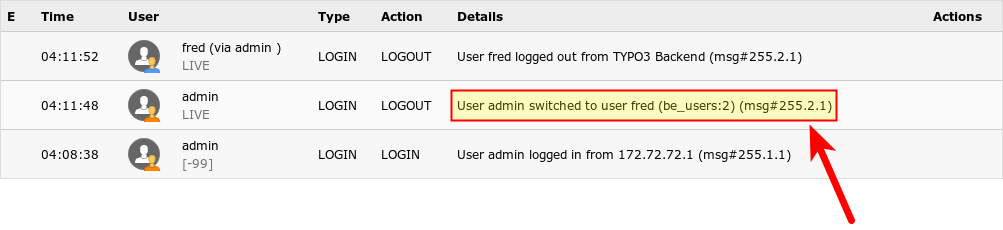
\includegraphics[width=0.90\linewidth]{ChangesForIntegrators/78432-SwitchUserActionLogMessage.png}
	\end{figure}

\end{frame}

% ------------------------------------------------------------------------------
% Feature | 83734 | Add support for current page in configcache
% Breaking | 88564 | PageTSconfig setting TSFE.constants removed
% Breaking | 88657 | Popup configuration in FormEngine dropped

\begin{frame}[fragile]
	\frametitle{Changements pour les intégrateurs}
	\framesubtitle{Changements TypoScript (1)}

	\begin{itemize}
		\item La propriété TypoScript \texttt{config.cache} supporte le mot-clé
			«~\texttt{current}~» référençant la page courante. Par exemple~: \newline
			\smaller\texttt{config.cache.all = fe\_users:current}\normalsize

		\item L'option de configuration Page/User TSconfig \texttt{TSFE.constants} est retirée.

			\begin{itemize}\smaller
				\item[\ding{228}] Incluez les conditions TypoScript dans la configuration et les constantes,
				et utilisez une configuration adéquate dans le fichier \texttt{ext\_localconf.php}.
			\end{itemize}

		\item Ces deux options de configuration de la taille des fenêtres popup sont retirées~:

			\begin{itemize}
				\item \texttt{options.popupWindowSize}
				\item \texttt{options.rte.popupWindowSize}
			\end{itemize}

	\end{itemize}

\end{frame}

% ------------------------------------------------------------------------------
% Breaking | 88640 | Database field sys_template.nextLevel and TypoScript sublevel inheritance removed
% Task | 88755 | Remove POST option from typolink.addQueryString

\begin{frame}[fragile]
	\frametitle{Changements pour les intégrateurs}
	\framesubtitle{Changements TypoScript (2)}

	\begin{itemize}
		\item Le champ de base de données \texttt{nextLevel} de la table
			\texttt{sys\_template} est retiré.

			\begin{itemize}\smaller
				\item[\ding{228}] Remplacez l'enregistrement (l'identifiant est enregistré dans le champ
					\texttt{nextLevel}) par une condition TypoScript pour les sous-pages.
					Par exemple~: \texttt{[tree.level > 1]}
			\end{itemize}\normalsize

		\item Les valeurs suivantes \textbf{ne sont plus permises}~:

			\begin{itemize}\smaller
				\item \texttt{typolink.addQueryString.method = POST}
				\item \texttt{typolink.addQueryString.method = GET,POST}
				\item \texttt{typolink.addQueryString.method = POST,GET}
			\end{itemize}\normalsize

			\begin{itemize}\smaller
				\item[\ding{228}] Changez les affectations TypoScript, Fluid et PHP par \texttt{GET}.
			\end{itemize}\normalsize

	\end{itemize}

\end{frame}

% ------------------------------------------------------------------------------
% Breaking | 87583 | Remove obsolete APC Cache Backend implementation
% Breaking | 87558 | Consolidate extbase caches

\begin{frame}[fragile]
	\frametitle{Changements pour les intégrateurs}
	\framesubtitle{Caches}

	% decrease font size for code listing
	\lstset{basicstyle=\tiny\ttfamily}

	\begin{itemize}
		\item Le framework de cache ne supporte plus \texttt{ApcBackend}

			\begin{itemize}\smaller
				\item[\ding{228}] Utilisez \textbf{APCu} en remplacement - notez le «~u~».
			\end{itemize}

\begin{lstlisting}
ANCIEN~:
$GLOBALS['TYPO3_CONF_VARS']['SYS']['caching']['cacheConfigurations']['rootline']['backend'] =
\TYPO3\CMS\Core\Cache\Backend\ApcBackend::class;

NOUVEAU~:
$GLOBALS['TYPO3_CONF_VARS']['SYS']['caching']['cacheConfigurations']['rootline']['backend'] = \TYPO3\CMS\Core\Cache\Backend\ApcuBackend::class;
	\end{lstlisting}

		\item Les caches Extbase \texttt{extbase\_reflection} et \texttt{extbase\_datamapfactory\_datamap}
			ont été consolidés et sont disponibles sous un seul cache nommé «~\texttt{extbase}~».

	\end{itemize}

\end{frame}

% ------------------------------------------------------------------------------
% Breaking | 87009 | Use multiple translation files by default in EXT:form

\begin{frame}[fragile]
	\frametitle{Changements pour les intégrateurs}
	\framesubtitle{Framework de formulaire}

	% decrease font size for code listing
	\lstset{basicstyle=\tiny\ttfamily}

	\begin{itemize}
		\item L'option suivante est renommée~:\newline
			\small\texttt{translationFile} \textrightarrow\hspace{0.1cm}\texttt{translationFiles}\normalsize
		\item Les fichiers de traduction par défaut sont déclarés en index 10~:

			\begin{itemize}
				\item \texttt{EXT:form/Resources/Private/Language/locallang.xlf}
				\item \texttt{EXT:form/Resources/Private/Language/Database.xlf}
			\end{itemize}

		\item Les formulaires personnalisés en configuration YAML doivent être mis à jour.

\begin{lstlisting}
ANCIEN~:
translationFile: path/to/locallang.xlf

NOUVEAU~:
translationFiles:
  20: path/to/locallang.xlf
\end{lstlisting}

	\end{itemize}

\end{frame}

% ------------------------------------------------------------------------------
% xxxxx | Cache Storage Type

\begin{frame}[fragile]
	\frametitle{Changements pour les intégrateurs}
	\framesubtitle{Type de stockage des caches (1)}

	\begin{itemize}

		\item TYPO3 fournit un système de cache flexible avec une configuration
			par défaut idéale dans la plupart des cas.
		\item Le type de stockage est configurable pour affiner les caches et
			augmenter les performances en fonction de l'environnement.

			\begin{itemize}
				\item Choisir le stockage en \textbf{base de données} pour un environnement classique
					ou si, par exemple, un système de fichiers réseau (NFS) est utilisé.
				\item Choisir le stockage sur le \textbf{système de fichiers} si, par exemple,
					une base de données distribuée est utilisée.
				\item Choisir des \textbf{paramètres de cache sur mesure} afin de configurer les types de stockage
					de façon indépendante.
			\end{itemize}

		\item Dans le cas d'installations plus complexes, des caches mémoire comme
			\href{https://redis.io/}{Redis (en)}
			ou
			\href{https://memcached.org/}{Memcached (en)} sont à étudier.

	\end{itemize}

\end{frame}

% ------------------------------------------------------------------------------
% xxxxx | Cache Storage Type

\begin{frame}[fragile]
	\frametitle{Changements pour les intégrateurs}
	\framesubtitle{Type de stockage des caches (2)}

	\begin{itemize}

		\item Backend~: \textbf{MAINTENANCE} \ding{223}\hspace{0.1cm}\textbf{Settings} \ding{223}\hspace{0.1cm}\textbf{Cache}:
		\end{itemize}

	\begin{figure}
		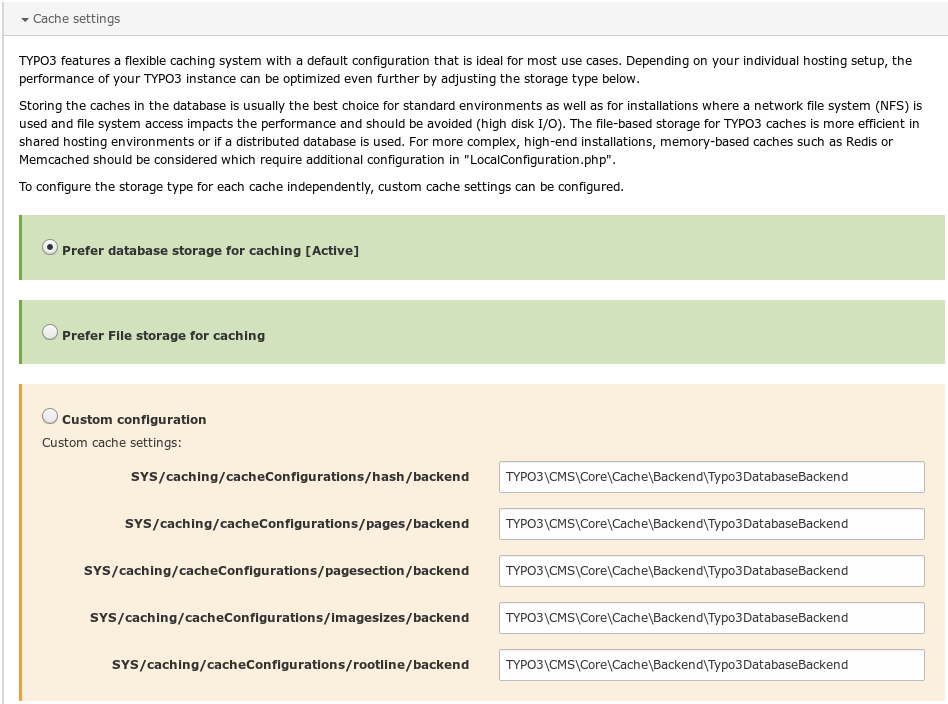
\includegraphics[width=0.60\linewidth]{ChangesForIntegrators/xxxxx-CacheStorageType.png}
	\end{figure}

\end{frame}

% ------------------------------------------------------------------------------
% 87499 | Drop extensions "taskcenter" and "sys_action" from core

\begin{frame}[fragile]
	\frametitle{Changements pour les intégrateurs}
	\framesubtitle{Centre de tâches et \texttt{EXT:sys\_action}}

	\begin{itemize}

		\item Les extensions système \texttt{EXT:taskcenter} et \texttt{EXT:sys\_action}
			ne font plus parties du cœur.

		\item Elles sont disponibles en extensions indépendantes depuis le
			\href{https://extensions.typo3.org/}{TER}
			et sur \href{https://github.com/FriendsOfTYPO3}{GitHub}.

		\item Gardez un œil sur l'
			\href{https://typo3.org/community/teams/typo3-development/initiatives/typo3-dashboard-initiative/}{initiative tableau de bord (en)}
			pour une nouvelle et meilleure approche.

	\end{itemize}

\end{frame}

% ------------------------------------------------------------------------------
% Feature | 88648 | Define Twitter Card Type In Page Properties
% Important | 86577 | Query parameters are now included in canonicalized URLs

\begin{frame}[fragile]
	\frametitle{Changements pour les intégrateurs}
	\framesubtitle{Divers (1)}

	% decrease font size for code listing
	\lstset{basicstyle=\tiny\ttfamily}

	\begin{itemize}

		\item Le type de Twitter Card est configurable.
			Cette option agit sur le rendu de la métadonnée \texttt{twitter:card} en FrontEnd.

\begin{lstlisting}
page {
  meta {
    twitter:card = summary_large_image
    twitter:card.replace = 1
  }
}
\end{lstlisting}

		\item Seuls les paramètres nécessaires pour le calcul du cHash sont inclus dans les URLs canoniques par défaut.
			Des paramètres de requête additionnels peuvent être configurés~:

\begin{lstlisting}
$GLOBALS['TYPO3_CONF_VARS']['FE']['additionalCanonicalizedUrlParameters'].
\end{lstlisting}

		\smaller
			Remarque~: N'ajoutez que les paramètres qui changent le contenu de la page. Dans le cas contraire les
			moteurs de recherche risquent de classifier vos pages en contenu dupliqué.
		\normalsize

	\end{itemize}

\end{frame}

% ------------------------------------------------------------------------------
% Breaking | 88681 | Import Of PHP Files In Import Export Files Removed
% Breaking | 88500 | RTE image handling functionality dropped
% Breaking | 81950 | Remove leftover workspaces unpublishing functionality

\begin{frame}[fragile]
	\frametitle{Changements pour les intégrateurs}
	\framesubtitle{Divers (2)}

	% decrease font size for code listing
	\lstset{basicstyle=\tiny\ttfamily}

	\begin{itemize}

		\item Lors de l'import de données XML de \texttt{EXT:impexp}, les motifs d'exclusion de
			fichier s'appliquent et rejettent en autres les fichiers PHP encapsulés.

		\item La gestion des images dans le RTE est intégralement retirée.
			Pour le support des images dans CKEditor, utilisez l'extension \texttt{EXT:rte\_ckeditor\_image} par exemple.

		\item Une propriété des espaces de travail pour dépublier les enregistrement est retirée de TYPO3 v10
			(y compris le champ de base de données \texttt{sys\_workspace.unpublish\_time}).
			Cette fonctionnalité fut désactivée dans TYPO3 v4.5 et n'est plus utilisée ou fournie depuis.

	\end{itemize}

\end{frame}

% ------------------------------------------------------------------------------
% Breaking | 88772 | JavaScript script tags omit type=text/javascript in HTML5
% Remove system extension EXT:rsaauth
% Remove system extension EXT:fe_edit

\begin{frame}[fragile]
	\frametitle{Changements pour les intégrateurs}
	\framesubtitle{Divers (3)}

	% decrease font size for code listing
	\lstset{basicstyle=\tiny\ttfamily}

	\begin{itemize}

		\item Lors du rendu en HTML5, les balises \texttt{<script>} n'incluent plus l'attribut \texttt{type="text/javascript"}.
		\item Pour le réactiver en frontend, utilisez le TypoScript ci-dessous~:

\begin{lstlisting}
page {
  includeJS {
    myfile = EXT:example/Resources/Public/JavaScript/myfile.js
    myfile.type = text/javascript
  }
}
\end{lstlisting}

		\item Les extensions système dépréciées suivantes sont retirées~:
			\begin{itemize}
				\item \texttt{EXT:rsaauth}
				\item \texttt{EXT:fe\_edit}
			\end{itemize}

	\end{itemize}

\end{frame}

% ------------------------------------------------------------------------------
